\documentclass[11pt]{exam}

% These are my most commonly-used LaTeX packages.
% You can add additional ones here as needed
\usepackage{amsmath,amsfonts,amssymb,amsthm}
\usepackage{fullpage}
\usepackage{times}
\usepackage{hyperref}
\usepackage{pdfsync}
\usepackage{microtype}
\usepackage{enumitem}
\usepackage{graphicx}

% Header.tex is a separate file 
%%% BLACKBOARD SYMBOLS

\newcommand{\C}{\ensuremath{\mathbb{C}}}
\newcommand{\D}{\ensuremath{\mathbb{D}}}
\newcommand{\F}{\ensuremath{\mathbb{F}}}
\newcommand{\G}{\ensuremath{\mathbb{G}}}
\newcommand{\J}{\ensuremath{\mathbb{J}}}
\newcommand{\N}{\ensuremath{\mathbb{N}}}
\newcommand{\Q}{\ensuremath{\mathbb{Q}}}
\newcommand{\R}{\ensuremath{\mathbb{R}}}
\newcommand{\T}{\ensuremath{\mathbb{T}}}
\newcommand{\Z}{\ensuremath{\mathbb{Z}}}
\newcommand{\QR}{\ensuremath{\mathbb{QR}}}

\newcommand{\Zt}{\ensuremath{\Z_t}}
\newcommand{\Zp}{\ensuremath{\Z_p}}
\newcommand{\Zq}{\ensuremath{\Z_q}}
\newcommand{\ZN}{\ensuremath{\Z_N}}
\newcommand{\Zps}{\ensuremath{\Z_p^*}}
\newcommand{\ZNs}{\ensuremath{\Z_N^*}}
\newcommand{\JN}{\ensuremath{\J_N}}
\newcommand{\QRN}{\ensuremath{\QR_{N}}}
\newcommand{\QRp}{\ensuremath{\QR_{p}}}

\newcommand{\Lap}{\text{Lap}}
\newcommand{\eps}{\epsilon}

%%% THEOREM COMMANDS

\theoremstyle{definition}

\newtheorem{theorem}{Theorem}%[section]

\newtheorem{lemma}[theorem]{Lemma}
\newtheorem{corollary}[theorem]{Corollary}
\newtheorem{proposition}[theorem]{Proposition}
\newtheorem{claim}[theorem]{Claim}
\newtheorem{fact}[theorem]{Fact}

\newtheorem{definition}[theorem]{Definition}
\newtheorem{conjecture}[theorem]{Conjecture}
\newtheorem{example}[theorem]{Example}
\newtheorem{protocol}[theorem]{Protocol}

\newtheorem{remark}[theorem]{Remark}
\newtheorem{note}[theorem]{Note}
\newtheorem{exercise}[theorem]{Exercise}

\newtheorem*{theorem*}{Theorem}
\newtheorem*{lemma*}{Lemma}
\newtheorem*{corollary*}{Corollary}
\newtheorem*{proposition*}{Proposition}
\newtheorem*{claim*}{Claim}
\newtheorem*{fact*}{Fact}
\newtheorem*{definition*}{Definition}
\newtheorem*{conjecture*}{Conjecture}
\newtheorem*{example*}{Example}
\newtheorem*{protocol*}{Protocol}

\newtheorem*{remark*}{Remark}
\newtheorem*{note*}{Note}
\newtheorem*{exercise*}{Exercise}

% equation numbering style
\numberwithin{equation}{section}

%%% GENERAL COMPUTING

\newcommand{\bit}{\ensuremath{\set{0,1}}}
\newcommand{\pmone}{\ensuremath{\set{-1,1}}}

% asymptotics
\DeclareMathOperator{\poly}{poly}
\DeclareMathOperator{\polylog}{polylog}
\DeclareMathOperator{\negl}{negl}

% probability/distribution stuff
\DeclareMathOperator*{\E}{E}
\DeclareMathOperator*{\Var}{Var}

% sets in calligraphic type
\newcommand{\calD}{\ensuremath{\mathcal{D}}}
\newcommand{\calF}{\ensuremath{\mathcal{F}}}
\newcommand{\calH}{\ensuremath{\mathcal{H}}}
\newcommand{\calX}{\ensuremath{\mathcal{X}}}
\newcommand{\calY}{\ensuremath{\mathcal{Y}}}

% types of indistinguishability
\newcommand{\compind}{\ensuremath{\stackrel{c}{\approx}}}
\newcommand{\statind}{\ensuremath{\stackrel{s}{\approx}}}
\newcommand{\perfind}{\ensuremath{\equiv}}

% font for general-purpose algorithms
\newcommand{\algo}[1]{\ensuremath{\mathsf{#1}}}
% font for general-purpose computational problems
\newcommand{\problem}[1]{\ensuremath{\mathsf{#1}}}
% font for complexity classes
\newcommand{\class}[1]{\ensuremath{\mathsf{#1}}}

% complexity classes and languages
\renewcommand{\P}{\class{P}}
\newcommand{\BPP}{\class{BPP}}
\newcommand{\NP}{\class{NP}}
\newcommand{\coNP}{\class{coNP}}
\newcommand{\AM}{\class{AM}}
\newcommand{\coAM}{\class{coAM}}
\newcommand{\IP}{\class{IP}}

%%% "LEFT-RIGHT" PAIRS OF SYMBOLS

% inner product
\newcommand{\inner}[1]{\langle{#1}\rangle}
\newcommand{\innerfit}[1]{\left\langle{#1}\right\rangle}
% absolute value
\newcommand{\abs}[1]{\lvert{#1}\rvert}
\newcommand{\absfit}[1]{\left\lvert{#1}\right\rvert}
% a set
\newcommand{\set}[1]{\{{#1}\}}
\newcommand{\setfit}[1]{\left\{{#1}\right\}}
% parens
\newcommand{\parens}[1]{({#1})}
\newcommand{\parensfit}[1]{\left({#1}\right)}
% tuple = alias for parens
\newcommand{\tuple}[1]{\parens{#1}}
\newcommand{\tuplefit}[1]{\parensfit{#1}}
% square brackets
\newcommand{\bracks}[1]{[{#1}]}
\newcommand{\bracksfit}[1]{\left[{#1}\right]}
% rounding off
\newcommand{\round}[1]{\lfloor{#1}\rceil}
% floor function
\newcommand{\floor}[1]{\lfloor{#1}\rfloor}
% ceiling function
\newcommand{\ceil}[1]{\lceil{#1}\rceil}
% length of a string
\newcommand{\len}[1]{\lvert{#1}\rvert}
\newcommand{\lenfit}[1]{\left\lvert{#1}\right\rvert}
% length of some vector, element
\newcommand{\length}[1]{\lVert{#1}\rVert}
\newcommand{\lengthfit}[1]{\left\lVert{#1}\right\rVert}

%%% VECTOR/MATRIX NOTATION

\newcommand{\veca}{\ensuremath{{\bf a}}}
\newcommand{\vecb}{\ensuremath{{\bf b}}}
\newcommand{\vecc}{\ensuremath{{\bf c}}}
\newcommand{\vecx}{\ensuremath{{\bf x}}}
\newcommand{\veczero}{\ensuremath{{\bf 0}}}

\newcommand{\matA}{\ensuremath{{\bf A}}}

%%% PSEUDOCODE

\newcommand{\pseudocode}[1]{
\ttfamily
\vbox{\begin{enumerate}
\renewcommand{\labelenumi}{}
\setlength\itemsep{-.3em}
{#1}
\end{enumerate}}
\rmfamily
}

%%% COLORED ANNOTATION

\usepackage[normalem]{ulem}
\usepackage{color}
\newcommand{\comment}[1]{{\color{blue} #1}}
\newcommand{\highlight}[1]{\colorbox{yellow}{#1}}
\newcommand{\grade}[1]{\vspace{0.2em}\noindent\comment{#1}}


%%% COMMANDS FOR QUIZES/HOMEWORKS/LABS/LECTURE NOTES


\newcommand{\assignmentheader}{
  \chead{\Large \textbf{\topic } }

  \rhead{\small
    \textbf{CMSC395 Final Project \\ \displaydate}}

  \lhead{\small {\bf  George, Joseph \\ Sisco, Marissa}}

  \setlength{\headheight}{20pt}
  \setlength{\headsep}{16pt}
  
  \headrule
}

\newcommand{\lectureheader}{
  \chead{\Large \textbf{\topic } }

  \rhead{\small
    \textbf{Lecture Notes \\ \displaydate}}

  \lhead{\small {\bf George, Joseph \\ Sisco, Marissa}}

  \setlength{\headheight}{20pt}
  \setlength{\headsep}{16pt}
  
  \headrule
}

\newcommand{\syllabusheader}{
  \chead{\Large \textbf{\topic } \\ {\small CMSC 395-01, Fall 2017}}

  \setlength{\headheight}{20pt}
  \setlength{\headsep}{16pt}
  
  \headrule
}


%% Thanks to Chris Peikert for portions of this file.
 

% Content for the file header, defined in Header.tex
\newcommand{\topic}{Generating Differentially Private
\\Laplacian Noise}
\newcommand{\displaydate}{September 26, 2017} 
\assignmentheader

% Only content between \begin{document} and \end{document} will be typeset
\begin{document} 
\bibliographystyle{alpha} 

\thispagestyle{head} % makes the file header appear on the first page


\section{Background}

The mathematical abstraction of the Laplacian mechanism differs greatly from its implementation in floating point representation.  In his paper, \textit{On Significance of the Least Significant Bits For Differential Privacy}, Mironov describes a new type of vulnerability present in implementations of the Laplacian mechanism. Specifically, this vulnerability results from the exploitation of the irregular distribution of the Laplacian mechanism resulting from finite precision and rounding effects of floating point operations.

Let's put this in more concrete terms by using an example of Laplacian sampling.  Say we have 10 double numbers, ranging from $x = 1/ \pi$ to $x+9 \cdot 2^{-54}$.  Applying the log function to each number in this set of 10 double numbers results in a transformation where some specific output numbers are more frequent than others.  Below is some code created to display this exact problem.  Notice how two numbers occur twice.

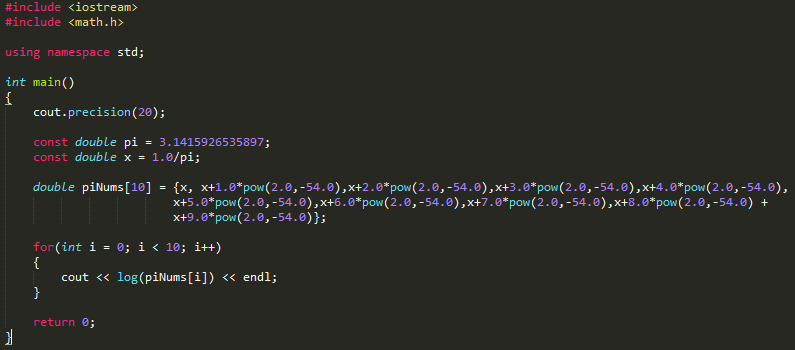
\includegraphics[width=\textwidth]{code.PNG}
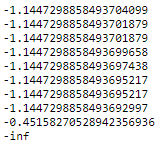
\includegraphics{result.PNG}

Similarly, using a different set of numbers, another thing can happen - the distribution is not evenly distributed and some output values from an interval become missing.  This "porous distribution," as Mirinov calls it, is what causes a breach in differential privacy.

To show this in concrete terms, consider the Laplacian mechanism $\tilde{f}(\cdot)_{\epsilon,p} = f(D) + Lap*_p (\Delta/\epsilon)$, where $p$ is the precision with which the uniform distribution over $(0,1)$ is sampled.  Let $\Delta = 1$, $f(D) = 0$, and $f(D') = 1$.  Consider the distribution of $\tilde{f}^*(D)_{1/3} = 0 + Lap*(3)$ and $\tilde{f}^*(D')_{1/3} = 1 + Lap*(3)$ around 1.5.  As it turns out, the output of the Laplacian mechanism results in some different values for $\tilde{f}^*(D)$ and $\tilde{f}^*(D')$.  For example, an output of $\tilde{f}^*(D)$ includes the value $1.5$ while $\tilde{f}^*(D')$ does not.  Similarly, $\tilde{f}^*(D')$ includes the value $1.5 + 2 \cdot 2^{-52}$, while $\tilde{f}^*(D)$ does not.  This means if the output of the Laplacian mechanism is $1.5 + 2 \cdot 2^{-52}$, the input database was $D'$ etc.  Thus, differential privacy is violated.

The paper \textit{Fast and Correctly Rounded Logarithms in Double Precision} by Dinechin, Lauder, and Mueller presents an algorithm to round floating point numbers precisely, to preserve differential privacy. As seen above, there are issues distributing noise with floating point values as they are not precise and can expose data. This new algorithm can provide accuracy up to $2^{-150}$ if needed. The main structure of this algorithm is comprised of 2 steps. The first step provides accuracy up to $2^{-60}$. It executes some operation on the float and then performs a rounding test. If the rounding test passes, this means there is no error and the algorithm can terminate with accuracy $2^{-60}$. There is a small chance, however, that there are inconsistencies in the values. In this case, the second step is implemented. It uses predefined libraries based on processor type to provide more accuracy. The output of this step will then be converted to a double precision number and is guaranteed to have accuracy of at least $2^{-150}$. By determining a way to integrate this algorithm into the snapping mechanism, we can preserve differential privacy with floating point numbers.  

\section{Objectives} 

Mironov proposed something called the \textit{snapping mechanism} to yield a differentially private mechanism by solving the issue explained above.  It works by tossing out the lower bits of the Laplacian noise result \textit{after} adding the noise to the query.  Previously, our differentially private mechanism was defined as $\tilde{f}(D) = f(D) + Lap*_p (\Delta/\epsilon)$.  Using Mironov's snapping mechanism, we now define it to be

\begin{align}
    \tilde{f}(D) \triangleq clamp_{B}(\lfloor clamp_{B}(f(D)) \oplus S \otimes \lambda \otimes LN(U^{*})  \rceil_{\Lambda}) 
\end{align}
\begin{itemize}
    \item $U^{*}$ is the uniform distribution over $\mathbb{D} \cap(0,1)$ such that each double number is output with probability proportional to its ulp
    \item $S$ is uniform over ${-1,+1}$
    \item $LN(\cdot)$ denotes a floating point implementation of the natural logarithm with exact rounding 
    \item Function $clamp_{B}(x)$ outputs: (1) $B$ if $x>B$, (2)$-B$ if $x<-B$, (3)$x$ otherwise
    \item $\Lambda$ is the smallest power of 2 (including negative powers) $\geq$ $\Lambda$ 
    \item $\lfloor \cdot \rceil_{\Lambda}$ round to the closest multiple of $\Lambda$ in $\mathbb{D}$ with ties resolved towards $+\infty$
\end{itemize}

The primary goal of this project is to create a software tool which generates Laplacian noise in a differentially private way by using the above mechanism defined by Mironov.  Additionally, we hope to be able to integrate this tool into a larger software framework that is used for querying databases.

\section{Deliverables}

\begin{enumerate}
    \item \textbf{DP Laplacian Noise Generator using Rust Language}: The goal here is to create a program that can use floating point numbers and generate Laplacian Noise in a way that preserves differential privacy. Rust will be used since it is a secure language that provides all the necessary tools we may need to complete the algorithm.
        
    \item \textbf{Integrated Software}: Once we have the basic algorithm completed, the next step is to determine what pre-existing frameworks we could potentially integrate the tool with. The purpose of this would be to ensure differential privacy with large database systems. After researching what possibilities exist, we would then modify our code so that the tool could work hand in hand with the framework.
    \item \textbf{Software Documentation}: Next we need to provide adequate documentation for our code. The goal would be for any user to be able to read and understand the code so they could use it with a database they may have. The documentation would include not only in code comments, but also a guide to explain how it works.
    \item \textbf{Software Bindings for C/Python (optional)}: Many projects related to this work are in C/Python. To make our code more accessible and flexible, we could add bindings so that it will work no matter which language it is to be used with. 
    \item \textbf{GUI for Software Tool (optional)}: If time allows, we could also create a GUI to make our tool more user friendly. This way, when users have a database, they would not need many software skills/terminal knowledge. The GUI would guide them through the process of adding noise to their database.
\end{enumerate}

\section{Project Timeline}
\begin{enumerate}
    \item \textbf{DP Laplacian Noise Generator using Rust Language}: October 16th
    \item \textbf{Integrated Software}:November 17th
    \item \textbf{Software Documentation}:November 30th
    \item \textbf{Presentation}: November 30th
    \item \textbf{Software Bindings for C/Python (optional)}: If time allows
     \item \textbf{GUI for Software Tool (optional)}: If time allows
\end{enumerate}
    

\bibliography{sample} % this loads the bibliography
\cite{M}
\cite{DLM}

\end{document}